\chapter{Introduction} \label{CHAP:Introduction}

\section{Motivation for High Performance Systems and Networks}

Some laws to remember:

\begin{description}
	\item[Moore's Law] For transistors: The amount of transistors doubles every two years. \\
	Similar observations can be found for Network Capacity, Storage, HDD Rates and more.
	
	\item[Wirth's law] Software becomes slower more rapidly than hardware becomes faster.
	
	\item[Gate's law] Speed of software halfs every 18 months.
	
	\item[May's law] Software efficiency halves every 18 months, compensating Moore's Law.
\end{description}

High performance and efficient network technologies are especially important for Embedded devices, HPCs, High Performance Routers and Real-time applications.\\

Therefore the lecture covers following subjects:

\begin{itemize}
	\item Micro-optimization in Chapter \ref{CHAP:MOPT}
	\item Performance Evaluation in Chapter \ref{CHAP:PERFEVAL}
	\item Algorithms and Datastructures and degree of freedom utilization in Chapters \ref{CHAP:PRINCIPLES} and following chapters.
\end{itemize}

\textbf{Examples of problems} this lecture tries to solve/highlight:\\

Different types of systems may have different bottlenecks, i.e., for

\textit{Network endnodes}:

\begin{itemize}
	\item Specialized for computations, General-purpose, i.e. endnode bottlenecks usually result from \textit{structure} and \textit{scale}
	\item \textbf{Structure}: \textit{Layered structure} of Operating systems, \textit{protection mechanisms} to protect the OS from other applications, core OS routines are written using \textit{general mechanisms} (Schedulers, Allocators). The combination of the different mechanisms may slow down networking software.
	
	\item \textbf{Scale}: Scaling factors of thousands of clients are possible, where many OSs simply don't use efficient enough data structures and algorithms, since they were designed for small amounts of connections.
\end{itemize}

In the book the following table shows a mapping between bottlenecks and solutions:

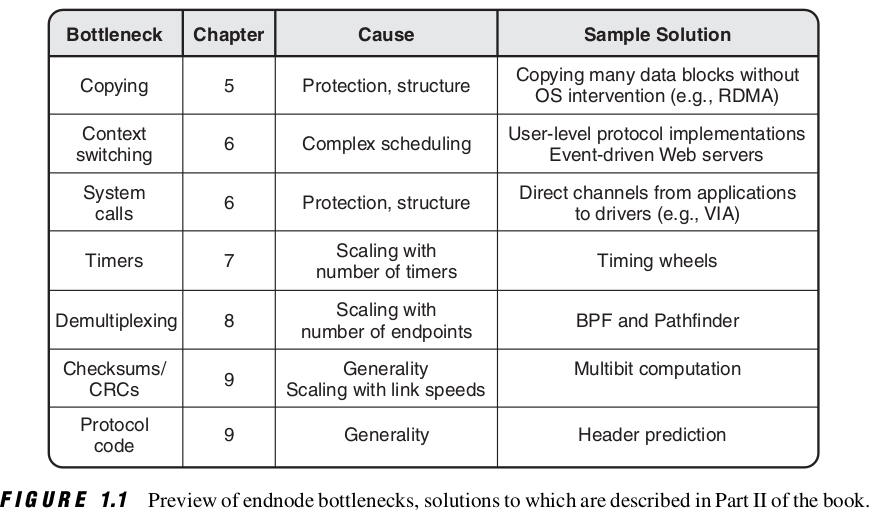
\includegraphics[width=.8\textwidth]{images/chap1/endnode_bottlenecks}

\textit{Router Bottlenecks}:

\begin{itemize}
	\item Special-purpose device, problems caused by \textit{scale} and \textit{services} and not structure
	
	\item {\textbf{Scale}: i.e., \textit{bandwidth scaling (from 1Gbps to 40Gbps)} and \textit{population scaling (growing number of endpoints)}}
	
	\item {\textbf{Services}: Many QOS (for instance \textit{network guarantees)} are/have been added over time, s.a., congestion control, protection during attacks, availability..}
\end{itemize}

Again, a mapping of bottlenecks to solutions provided by the book:

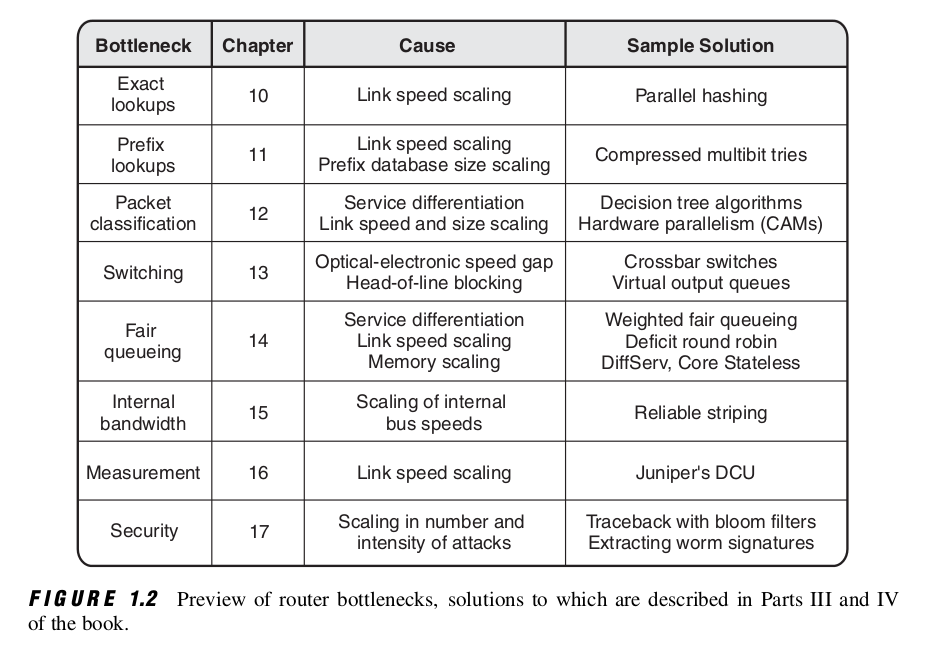
\includegraphics[width=.8\textwidth]{images/chap1/router_bottlenecks}

Nowadays, routers provide \textit{service differentation}, i.e., handling different packets differently, depending on the offered services, which requires \textit{packet classification}.

\section{Warmup-Example: Scenting an evil packet}

\textbf{Problem:} An attacker tries to include malicious data in a packet, that is later executed on the target system. How? If the target system does not allocate enough buffer space and does not check
for overflow, malicious code can be performed on the target system.

\textbf{Solution:} Implemenation of a pre-filter by estimating what a packet "usually" \ looks like, i.e., estimating the frequencies of bytes in a packet.

Issues regarding the implementation:

\begin{itemize}
	\item Fast counting of characters/bytes in a packet
	\item Estimation of non-malicious packet
	\item Estimating such that false negatives don't appear. False positives are ok, since they have to go through the IDS.
\end{itemize}

\textbf{Stage 1 - Strawman Soltuion:} naive approach, consists of an array $C$ with 256 elements, one for each byte. For incoming packets $\rightarrow$ iteration through data, increment $C$ at position of byte.
A threshold array $T$ is used to estimate whether $C$ is out of the ordinary. In formulas:

$$C[j] \geq L \cdot T[j] , L = packet \ length, j \in \mathbb{N}, 0 \leq j \leq 255$$

The example in the book only applies for HTTP headers, i.e., the check is only done on the URL and is only initiated if a HTTP Header is recognized.

Usually packets are incoming at high speed and ideally they are processed before the next one arrives. This is called \textbf{wire speed processing}!

Since intialization of arrays is static we have 1 write + 1 read per $C$ and 1 read per $T$ we have at least 768 operations per packet. However, a packets minimum size is 40 bytes and in this case we have a great overhead.

\textbf{Stage 2 - Thinking Algorithmically:} Only keep track of the largest ratio of character count to threshold. I.e., $C[k]/T[k] = MAX$ is being memorized. New characters still increment $C[i]$ and if $C[i]/T[i] > MAX$, max is replaced. The process can stop if $MAX > L$.

\textbf{Stage 3 - Exploit Hardware:} The last loop is eliminated, but we still have division. Idea: approximate threshold by a power of 2, as they are estimates anyway. Then shifting can be used instead of division.
For instance 1/29 becomes 1/32. Shift values are now stored instead of thresholds themselves. Now $C[i]$ is incremented an the check is $C[i] << T[i] > MAX$.

Still one read + write for $C$ and one read for $T$ is required, which is now the new bottleneck instead of computation itself. By combining the counter and threshold into one word only one read is required (for instance using a union).


\textbf{Stage 4 - Cleaning Up:} Intialization is still done for 256 values. Hence, lazy init. is preferable, since for packets of 40 bytes, less operations are needed. Idea:

Keep a register $G$ (3-bit as we already have 29 bit for $C$ and $T$ and therefore 3 left). When a new packet is incoming increment a global register $g mod 8$. When $C[i]$ is incremented, check if $G[i] == g$, if that is not the case, we know that $i$ was not used in this turn and can be initialized to $1$, otherwise it's incremented.


























